\documentclass[a4paper,oneside,12pt]{amsart}

%\usepackage[spanish, activeacute]{babel}
\usepackage[utf8]{inputenc}
%\usepackage[latin1]{inputenc}
\usepackage{latexsym}
\usepackage{multicol}
\usepackage{enumerate}
\usepackage{enumitem}
\usepackage[heightrounded]{geometry}
\geometry{top=2cm,bottom=2cm,left=2cm,right=2cm}
\usepackage{graphicx}
\usepackage{tikz}
\usetikzlibrary{graphs, graphs.standard}
\usepackage{amssymb}
\usepackage{tikz-network}

\DeclareMathOperator{\cond}{cond}
\DeclareMathOperator{\Id}{Id}
\DeclareMathOperator{\re}{Re}
%\DeclareMathOperator{\im}{Im}
\newcommand{\I}{\mathbb{I}}
\newcommand{\R}{\mathbb{R}}
\newcommand{\Q}{\mathbb{Q}}
\newcommand{\C}{\mathbb{C}}
\newcommand{\Z}{\mathbb{Z}}
\newcommand{\N}{\mathbb{N}}
\DeclareMathOperator{\im}{Im}

\newcommand{\nombremateria}
{Investigaci\'on Operativa}
\newcommand{\nombrecuatrimestre}
    {Segundo cuatrimestre de 2025}
\newcommand{\numeroparcial}
    { Recuperatorio del Tercer Parcial }
\newcommand{\fecha}
    {19 de Diciembre de 2025}
\newcommand{\numerotema}
    {\bf 1}

%\oddsidemargin -1cm \evensidemargin -1cm \textwidth 17.5cm
%topmargin 1.2cm \textheight 25cm
%\setlength{\textheight}{25cm}

\def \ds{\displaystyle}
\theoremstyle{definition}
\newtheorem{quest}{Ejercicio}
\thispagestyle{empty}

\begin{document}

\hfill \hfill
\begin{tabular}[c]{|c|c|c|c|}
\hline 
1 & 2 & 3 & Calificaci\'on \\ \hline \hline
\hspace{1.2 cm} & \hspace{1.2 cm} & \hspace{1.2 cm} &\hspace{1.5 cm} \\
\hspace{1.2 cm} & \hspace{1.2 cm} & \hspace{1.2 cm} &\hspace{1.5 cm} \\ \hline

\end{tabular}

\vspace{-1cm}

\noindent Nombre y apellido:

\vspace{0.2cm}

\noindent Número de libreta:

\noindent \hrulefill 

\smallskip
\renewcommand{\baselinestretch}{1.1}

\begin{center}
	\large \textbf{\nombremateria} 
	
	\numeroparcial -- \fecha
\end{center}

\begin{center}
\textbf{Entregue todos los ejercicios en hojas separadas.}
\end{center}

\vspace{.6cm}
\renewcommand{\theenumi}{\textbf{\arabic{enumi}}}

%%% EMPIEZA EL EJERCICIO 1 %%%

\begin{quest}\verb|[3.5 pts.]|
Demostrar las siguientes afirmaciones. Cada ítem se puede demostrar individualmente, no es necesario utilizar el
resultado de los demás.
%\noindent
\begin{enumerate}[label=\alph*)]
    \item \verb|[0.5 pts.]| Sea $G$ un grafo tal que el grado de todo vértice es $r$. Probar que la cantidad de
    aristas de $G$ es múltiplo de $r$.
    \item \verb|[1.25 pts.]| Para $G=(V,E)$ conexo, probar que la arista $e$ pertenece a todo árbol generador
    mínimo de $G$ si y sólo existe $V'\subsetneq V$ tal que $e$ es la única arista de peso mínimo que conecta $V'$
    con $V-V'$.
    \item \verb|[0.5 pts.]| Sea $G=(V,E)$ conexo y bipartito con bipartición $V=V_1\cup V_2$. ¿Es cierto que si
    todos los vértices de $V_1$ tienen grado par entonces $G$ admite un circuito euleriano?
%    \item Sea $G$ un grafo con $n$ vértices. Supongamos que
%    $|E|\geq \frac{(n-2)(n-3)}{2}+2 $. Demostrar que $G$ tiene un camino Hamiltoniano.
    \item \verb|[1.25 pts.]| Llamamos \textit{circunferencia} de un grafo $G$ al ciclo de menor tamaño
    \footnote{El tamaño de un ciclo
    viene dado por su cantidad de aristas}. Sea $G$ un grafo planar conexo tal que cada arista pertenece a exactamente dos
    regiones y $k \geq 3$ su circunferencia. Demostrar que $|E|\leq \frac{k(|V|-2)}{k-2}$.\\
    \textbf{Sugerencia:} probar que $k|R| \leq 2|E|$ y usar la fórmula de Euler

\end{enumerate}
\end{quest}

%%% TERMINA EL EJERCICIO 1 %%%

%%% EMPIEZA EL EJERCICIO 2 %%%


\begin{quest}\verb|[3.5 pts.]|
Sea $G$ el siguiente grafo:

    \begin{center}
        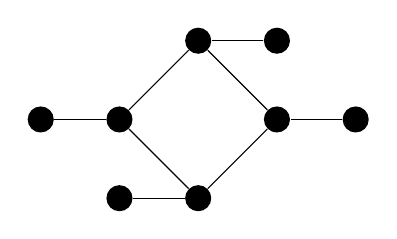
\begin{tikzpicture}
            \graph[nodes={fill=black, circle}, empty nodes, clockwise] { subgraph C_n [V={1,2,3,4}, clockwise];
            5[at={(1,1)}] -- {1};
            6[at={(-2, 0)}] -- {4};
            7[at={(-1, -1)}] -- {3};
            8[at={(2, 0)}] -- {2};
%            8[at={(0, -1.5)}] -- {3,4};
%            9[at={(-1.3, -0.4)}] -- {4,5};
%            10[at={(-1, 1.1)}] -- {5,1};
            };

        \end{tikzpicture}
    \end{center}

    \begin{enumerate}[label=\alph*)]
        \item \verb|[0.5 pts.]| Calcular el polinomio cromático de $G$. Justificar.\\
        \textbf{Sugerencia:} recordar que el polinomio cromático de $C_n$ es $P(k)=(k-1)^n + (-1)^n(k-1)$
        \item \verb|[0.75 pts.]| Calcular el número cromático de $G$ y cuántos posibles coloreos hay con $\chi(G)$
        colores. Justificar.
        \item \verb|[0.75 pts.]| Calcular el índice cromático de $G$. Justificar.
        \item \verb|[0.5 pts.]| Decimos que un grafo es circular si se lo puede representar mediante cuerdas en un
        círculo, de manera tal que cada cuerda representa un vértice y dos cuerdas se intersecan si y solo si los
        correspondientes vértices son adyacentes en $G$. Por ejemplo:
             \begin{center}
            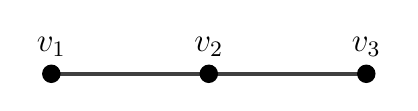
\begin{tikzpicture}
                \SetVertexStyle[FillColor=black, MinSize=0.7]
                \Vertex[label=$v_1$, position=above, fontsize=\large, x=0, y=0]{s1}
                \Vertex[label=$v_2$, position=above, fontsize=\large, x=2, y=0]{s2}
                \Vertex[label=$v_3$, position=above, fontsize=\large, x=4, y=0]{s3}
                \Edge(s1)(s2)
                \Edge(s2)(s3)
            \end{tikzpicture} \hspace{2cm}
        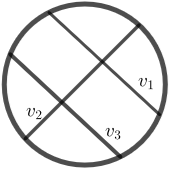
\includegraphics[scale=0.55]{grafo_circular_2}
        \end{center}
        ¿Es $G$ un grafo circular? Justificar.
        \item \verb|[0.5 pts.]|
        Un grafo se dice ``de intervalos" si se pueden representar sus vértices a través de intervalos abiertos
        en la recta real de modo de que cada intervalo está
        asociado a un vértice y dos vertices son adyacentes si y solo si los intervalos se intersecan. Por ejemplo:
        \begin{center}
            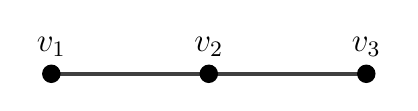
\begin{tikzpicture}
                \SetVertexStyle[FillColor=black, MinSize=0.7]
                \Vertex[label=$v_1$, position=above, fontsize=\large, x=0, y=0]{s1}
                \Vertex[label=$v_2$, position=above, fontsize=\large, x=2, y=0]{s2}
                \Vertex[label=$v_3$, position=above, fontsize=\large, x=4, y=0]{s3}
                \Edge(s1)(s2)
                \Edge(s2)(s3)
            \end{tikzpicture} \hspace{2cm}
            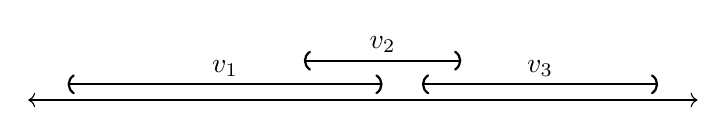
\begin{tikzpicture}
                    \draw[<->] (0,0) -- (8.5,0);
                    \draw[(-), thick] (0.5,0.2) -- (4.5,0.2);
                    \node (v1) at (2.5, 0.4) {$v_1$};

                    \draw[(-), thick] (3.5,0.5) -- (5.5,0.5);
                    \node (v1) at (4.5, 0.7) {$v_2$};

                    \draw[(-), thick] (5,0.2) -- (8,0.2);
                    \node (v1) at (6.5, 0.4) {$v_3$};

                \end{tikzpicture}
        \end{center}
        ¿Es $G$ un grafo de intervalos? Justificar.
        \item \verb|[0.5 pts.]| Un grafo se dice ``arco-circular'' si es el grafo intersección de arcos abiertos
        alrededor de un círculo, es
        decir, si se pueden representar sus vértices a través de dichos arcos de modo de que cada arco está
        asociado a un vértice y dos vertices son adyacentes si y solo si los arcos se intersectan. Por ejemplo:
        \begin{center}
            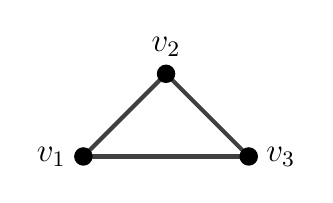
\begin{tikzpicture}[scale=0.7]
                \SetVertexStyle[FillColor=black, MinSize=0.7]
                \Vertex[label=$v_1$, position=left, fontsize=\large, x=0, y=0]{v1}
                \Vertex[label=$v_2$, position=above, fontsize=\large, x=1.5, y=1.5]{v2}
                \Vertex[label=$v_3$, position=right, fontsize=\large, x=3, y=0]{v3}
%                \Vertex[label=$v_4$, position=below, fontsize=\large, x=1.5, y=-1.5]{v4}
                \Edge(v1)(v2)
                \Edge(v2)(v3)
                \Edge(v3)(v1)
%                \Edge(v4)(v1)
            \end{tikzpicture}\hspace{2cm}
%        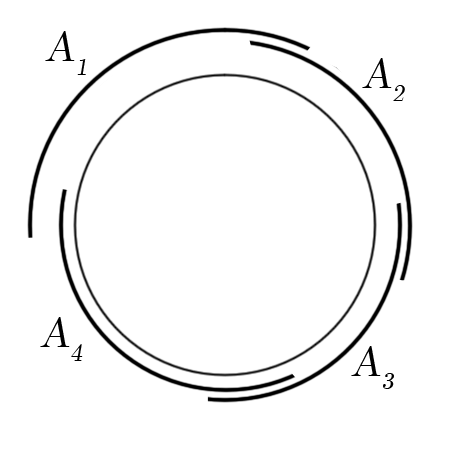
\includegraphics[scale=1]{../2021/Imagenes/arc.png}
            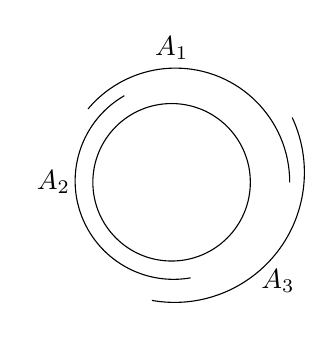
\begin{tikzpicture}
                \draw (0,0) circle(1);
                \draw (1.5,0) arc (0:140:1.45);
                \draw (-0.6,1.1) arc (120:280:1.25);
                \draw (-0.25,-1.5) arc (260:385:1.65);

                \node at (-1.5,0) (A) {$A_2$};
                \node at (0,1.7) (B) {$A_1$};
                \node at (1.35,-1.25) (B) {$A_3$};
            \end{tikzpicture}
        \end{center}
        ¿Es $G$ un grafo arco-circular? Justificar.
%        \item \verb|[0.5 pts.]| Un grafo es círculo si es el grafo intersección de cuerdas dentro de un círculo.
    \end{enumerate}
\end{quest}

%%% TERMINA EL EJERCICIO 2 %%%

%%% EMPIEZA EL EJERCICIO 3 %%%

\begin{quest}
    \verb|[3 pts.]| Una empresa opera una red distribuida de equipos de trabajo encargados de ejecutar instrucciones
    críticas de mantenimiento. Cada equipo puede retransmitir la instrucción a otros equipos pero algunas conexiones
    son poco confiables. Si existe un canal de comunicación entre el equipo $i$ y el equipo $j$, se conoce la
    probabilidad $p_{ij}\in(0,1]$ de que la transmisión desde $i$ a $j$ sea existosa y, análogamente, se conoce
    $p_{ji}\in(0,1]$ la probabilidad de que la transmisión desde $j$ a $i$ se lleve a cabo correctamente.

    Además, algunos equipos son nodos
    críticos: si la instrucción pasa por ellos, la retransmisión exitosa no está asegurada debido a diferentes
    factores como interpretación incorrecta o incompatibilidad técnica. Sea $C$ el
    conjunto de nodos críticos, para cada $i\in C$ se conoce la probabilidad $q_i\in (0, 1)$ de que transmitan
    correctamente la información.

    A continuación se muestra un ejemplo de red de equipos. El equipo $0$ corresponde a la casa matriz de la
    empresa, los equipos sombreados son los nodos críticos y dos equipos están conectados si y solo si existe un
    canal de comunicación entre ellos:

        \begin{center}
        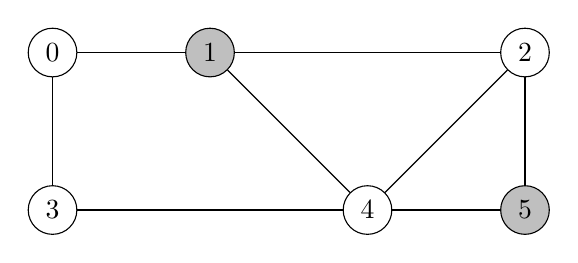
\begin{tikzpicture}
            \node[circle, draw] (0) at (0,0) {0};
            \node[circle, draw, fill=gray!50!white] (1) at (2,0) {1};
            \node[circle, draw] (2) at (6,0) {2};
            \node[circle, draw] (3) at (0,-2) {3};
            \node[circle, draw] (4) at (4,-2) {4};
            \node[circle, draw, fill=gray!50!white] (5) at (6,-2) {5};

            \draw (0) -- (1);
            \draw (1) -- (2);
            \draw (1) -- (4);
            \draw (2) -- (5);
            \draw (0) -- (3);
            \draw (3) -- (4);
            \draw (4) --  (5);
            \draw (4) --  (2);
        \end{tikzpicture}
    \end{center}

    Se puede asumir que todas las probabilidades son independientes entre sí. Por ejemplo, la probabilidad de que
    una instrucción se transmita correctamente desde el equipo $0$ al equipo $2$ mediante la ruta $0\rightarrow 1\rightarrow 2$ es de
    $p_{01}\cdot q_1 \cdot p_{12}$.

    Para una red de equipos en general, la
    empresa desea determinar los rutas de transmisión de instrucciones desde la central (equipo de trabajo $0$) al
    resto de los equipos maximizando la probabilidad de éxito. Modelar el problema como un problema
    de grafos y proponer uno de los algoritmos vistos en clase para resolverlo en tiempo polinomial.

\end{quest}

%%% TERMINA EL EJERCICIO 3 %%%

%%% TERMINA EL PARCIAL %%%



\end{document}

